\section{Finances}

\subsection{Basic Costs}
The first step in identifying what funding would be required was to identify the most basic costs for the business. They are presented in the following figure.

\begin{figure}[ht!]
\centering
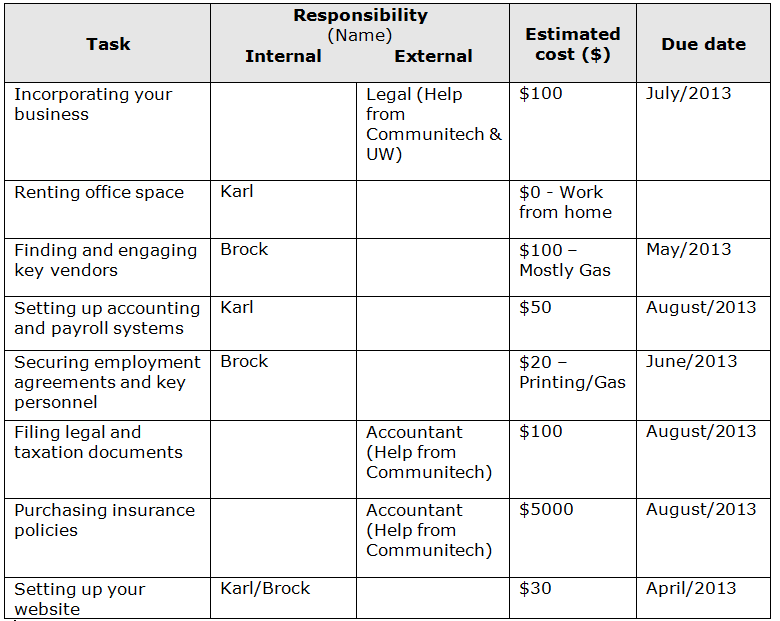
\includegraphics[width=150mm]{images/TaskList.png}
\caption{Task Breakdown}
\label{tasks}
\end{figure}

\subsection{Growth Plan}
The stepping stones described in the Go-to-Market Strategy section of the plan are reiterated in the following financing roadmap. The necissary funding required for each step is presented underneath the appropriate stepping stone.

\begin{figure}[ht!]
\centering
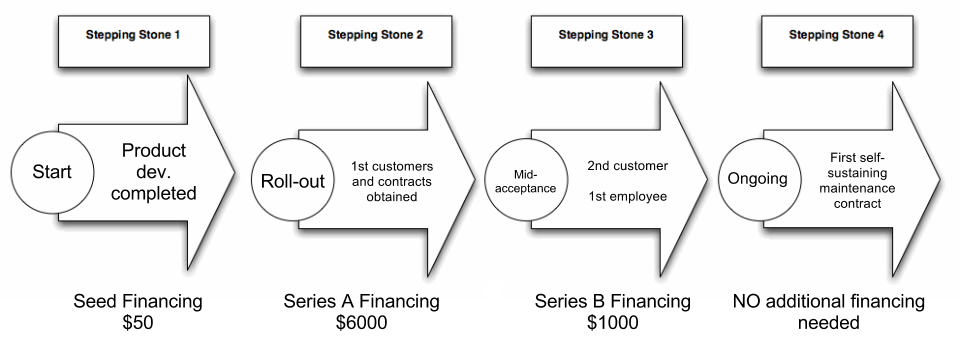
\includegraphics[width=150mm]{images/MSCI454-FinancingRoadmap.png}
\caption{Financing Roadmap}
\label{steppingStones}
\end{figure}
 
Initially only \$50 seed financing will be required. This will cover meanial costs associated with working from home and developing the product. This assumes our team is volunteering their hours to develop the product.

Series A financing entails purchasing the required server space to host our application for our client to access it before we have started to receive revenue. The rest of the costs associated with this stage of financing are associated with travel to and from client meetings.

Series B financing is again to cover small costs that have to do with client meetings. All necissary expansion costs are covered by the revenue obtained by initial client membership fees.

During the ongoing phase, {\bf Acknowledgements} is self-sustaining based on revenue and does not need additional financing.

\subsection{Pitch Scenarios}
Ideally, you can provide two sales scenarios
based on a high and low case to show the sensitivity and range for your plan.

\subsection{Accounting}
The {\bf Acknowledgements} Balance Sheet for the first year is presented in teh following table. This Balance Sheet does not assume that the development hours provided by the team are volunteered for free.

\begin{table}[ht]
\caption{The Balance Sheet} % title of Table
\centering % used for centering table
\begin{tabular}{| l c c c |} % centered columns (4 columns)
\hline
Item of Service & Cost per Unit (\$) & Quantity in First Year & Cost for First Year (\$) \\
\hline % inserts single horizontal line
Office (Work from home) & & & \\
Computers & 1500 & 2 & 3000 \\
Internet Service & 60 & 12 & 720 \\
Office Supplies & 300 & 1 & 300 \\
Printer & 150 & 1 & 150 \\
 &   &   &   \\
Product &   &   &   \\
Web Hosting & 150 & 1 & 150 \\
Development Hours & 30 & 1500 & 45000 \\
  &   &   &   \\
Client Meetings &   &   &   \\
Lunches & 50 &  50 & 2500\\
Gas & 50 & 20 & 1000 \\
 &   &  &   \\
Total &   &   & 52820 \\

\hline %inserts single line
\end{tabular}
\label{balanceSheet} % is used to refer this table in the text
\end{table}

